%!TEX root = ../dokumentation.tex
\chapter{Grundlagen Laserentferungsmessung}

\section{Lichtlaufzeitmessung}
Das Grundprinzip der Lichtlaufzeitmessung oder auch \acf{ToF} (Abbildung: \ref{tof}), bezieht sich auf die Zeit, welche ein ausgesandter Lichtimpuls benötigt bis er wieder am Sender eintrifft.\\
\begin{figure}[H]
	\centering
	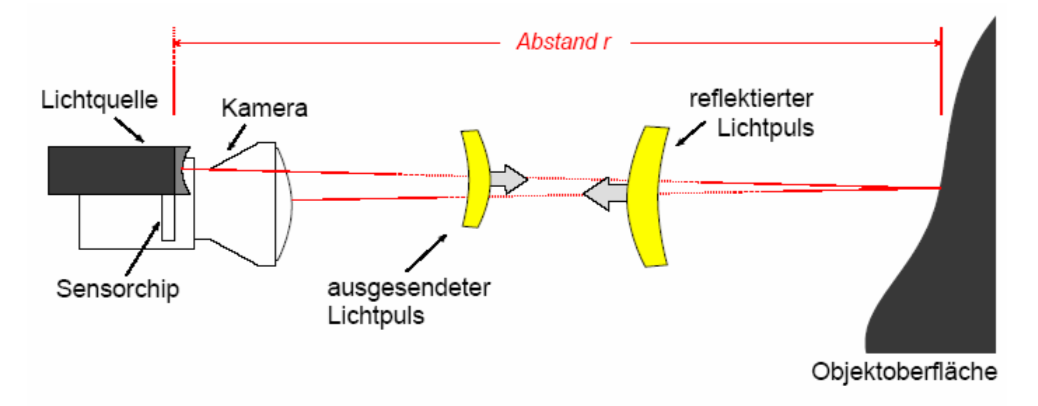
\includegraphics[width=0.75\textwidth]{images/GrundlagenLaserentfernungsmessung/ToF}
	\caption{\ac{ToF} Prinzip \cite{ToF_TUBerlin}}
	\label{tof}
\end{figure}
\section{Phasenverschiebung}
Das Phasenverschiebungsverfahren macht sich zu nutzen, dass bei einer ausgesandten Elektromagnetischen Welle die Phase immer größer wird bei steigender Entfernung. Durch Aussenden verschieden Frequentierter Wellen kann dann die Phasenverschiebung der Wellen bestimmt werden und daraus die Entfernung.\\

\section{Triangulation}